\subsubsection{Kommunikationsmodul}
Abbildung \ref{fig:kommunikationsmodul} zeigt die verschiedenen Schnittstellen, über welche Daten mit der Umgebung (User) und \textit{MCU} ausgetauscht werden können.\\

\begin{figure}[h]
	\centering
	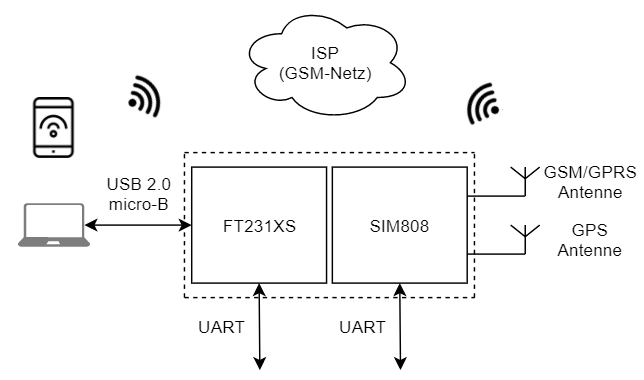
\includegraphics[scale=0.7]{graphics/Konzeptdiagramme/Kommunikationsmodul.PNG}
	\caption{Kommunikationsmodul}
	\label{fig:kommunikationsmodul}
\end{figure}

Der User hat die Möglichkeit, per Computer die Daten der Wetterstation direkt abzufragen, oder aber auch über sein Mobilfunktelefon mittels SMS. Dafür benötigt der User eine zusätzliche SIM-Karte vom lokalen Internet Service Provider\footnote{Z.B. Swisscom, Salt, Sunrise, usw.} (ISP) für die Wetterstation, welche er dann mittels Computer über die serielle Schnittstelle entsperren kann.\\
